The $2*n$ Fig ~\ref{fig:2t10} homogeneous mesh network processes load $L$ and $L$ originates $P_{0}$.  

\begin{figure}[!ht]
\centering
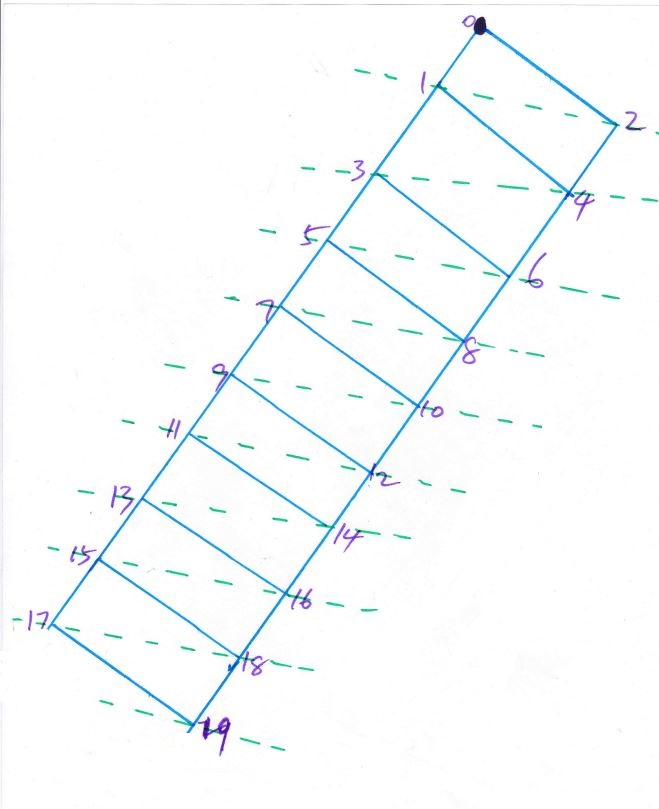
\includegraphics[width=0.6\columnwidth]{figure/2t10.JPG}
\caption{2*n (n = 10) mesh network and the workload happens on $P_{0}$}
\label{fig:2t10}
\end{figure}

Load a distribution from $P_{0}$ to $P_{1}$ and $P_{2}$ via virtual cut-through.  After $P_{1}$ and $P_{2}$ finish receiving load from link $0-1$ and $0-2$, they will be used to forward load to $P_{3}$ and $P_{4}$ and so on.

The equations are presented as:
\begin{empheq}[left=\empheqlbrace]{align}
\alpha_{0} \omega T_{cp} = T_{f, m}\\
\alpha_{1} \omega T_{cp} = T_{f, m}\\
\alpha_{2} \omega T_{cp} = T_{f, m}\\
\alpha_{1}zT_{cm} + \alpha_{3}\omega T_{cp} = T_{f, m}\\
\alpha_{2}zT_{cm} + \alpha_{4}\omega T_{cp} = T_{f, m}\\
(\alpha_{1} + \alpha_{3})zT_{cm} + \alpha_{5}\omega T_{cp} = T_{f, m}\\
\vdots \\
(\alpha_{1} \cdots + \alpha_{2 \times n - 1})zT_{cm} +\alpha_{2 \times n - 1} \omega T_{cp} = T_{f, m}\\
\alpha_{0} + \cdots + \alpha_{2 \times n - 1} = 1\\
\sigma = \frac{zT_{cm}}{\omega T_{cp}}\\
0 < \sigma < 1 \\
0 < \alpha_{0} \leq 1\\
0 \leq \quad \alpha_{1} \quad \alpha_{2} \quad  \cdots  \quad \alpha_{2 \times n - 1} < 1
\end{empheq}


The flow matrix closed-form is shown:
\begin{equation}
{
\left[ \begin{array}{ccccccc}
1 & 2 & 2 & \cdots & 2 & 2 & 1\\
1 & -1 & 0 & \cdots& 0 & 0 & 0\\
0 & \sigma-1 & 1 & \cdots & 0 & 0 & 0 \\
0 & \sigma-1 & \sigma & 1 & 0 & \cdots & 0 \\
0 & \sigma-1 & \sigma & \sigma & 1 & 0 & 0 \\
\vdots & \vdots & \vdots  &   \vdots & \ddots & \ddots\\
0 & \sigma-1 & \sigma & \cdots & \sigma & \sigma & 1
\end{array} 
\right ]} \times \left[ \begin{array}{c}
\alpha_{0} \\
\alpha_{1} \\
\alpha_{3} \\
\alpha_{5} \\
\vdots \\
\alpha_{2 \times n - 3}\\
\alpha_{2 \times n - 1}
\end{array} 
\right ] = \left[ \begin{array}{c}
1 \\
0 \\
0 \\
0 \\
\vdots \\
0 \\
0
\end{array} 
\right ]
\end{equation}

According to the \textbf{\textit{Cramer's rule}},the explicit solution for the group of equations is:
\begin{empheq}[left=\empheqlbrace]
{align}
\alpha_{i} = \left |\frac{\det A^{\star}_{i}}{\det A}\right |
\end{empheq}
where $A^{\star}_{i}$ is the matrix formed by replacing the $i$-th column of A by the column vector b.\\
Especially,
\begin{equation}
{
A^{\star}_{0} = \left[ \begin{array}{ccccccc}
1 & 2 & 2 & \cdots & 2 & 2 & 1\\
0 & -1 & 0 & \cdots& 0 & 0 & 0\\
0 & \sigma-1 & 1 & \cdots & 0 & 0 & 0 \\
0 & \sigma-1 & \sigma & 1 & 0 & \cdots & 0 \\
0 & \sigma-1 & \sigma & \sigma & 1 & 0 & 0 \\
\vdots & \vdots & \vdots  &   \vdots & \ddots & \ddots\\
0 & \sigma-1 & \sigma & \cdots & \sigma & \sigma & 1
\end{array} 
\right ]}
\end{equation}

$$\alpha_{0} = \left |\frac{\det A^{\star}_{0}}{\det A} \right |$$
$$\det A^{\star}_{0} = -1$$

The equivalence inverse processing speed :
$$T_{f,n} = 1*w_{eq}*T_{cp}$$
$$w_{eq} = \alpha_{0}*w$$

Finally, the speedup is:
$$Speedup = \frac{T_{f, 0}}{T_{f, n}}= \frac{\omega T_{cp}}{\alpha_{0}\omega T_{cp}} = \frac{1}{\alpha_{0}} =  \left|-\det A\right|$$.
